\chapter{实验结果及应用}
\section{数据集描述与环境说明}
算法会在会在第\label{cha:data}节提供的数据集上进行验证。实验的硬件环境如表\ref{tab:predicEnHard}所示。软件环境如表\ref{tab:preicEnSO}所示。
\begin{table}[H]
    \caption{产气量预测实验硬件环境}
    \label{tab:predicEnHard}
    \begin{tblr}{hlines,vlines,
        columns = {valign=m,co=-1},
        rows    = {halign=c},}
        处理器 & 显卡 & 内存 & 硬盘 \\
        Inter(R) Xeon(R) Silver 4261 cpu @ 2.10Hz & GeForce RTX 3090 & 256G & 1T \\
    \end{tblr}
\end{table}
\begin{table}[h]
    \caption{产气量预测实验软件环境}
    \label{tab:preicEnSO}
    \begin{tblr}{hlines,vlines,
        columns = {valign=m,co=-1},
        rows    = {halign=c},}
        操作系统 & 开发环境 & Anaconda & Python \\
        Windows 10 & Pycharm & 4.12.0 & 3.9 \\
    \end{tblr}
\end{table}
\section{气井分类实验结果}
由第三章可知,根据结合RFM与核密度的气井分类算法,气井将被分为四类,每一类的结果如表\ref{tab:everyclassnumber}所示。图\ref{fig:classResusca}为分类结果的展示。
\begin{table}[H]
    \caption{气井分类结果展示表}
    \label{tab:everyclassnumber}
    \begin{tblr}{hlines,vlines,
        columns = {valign=m,co=-1},
        rows    = {halign=c},}
        气井类别 & 数量 \\
        活跃高价值 & 447 \\
        不活跃高价值 & 266 \\
        活跃一般价值 & 332 \\
        不活跃一般价值 & 24 \\
    \end{tblr}
\end{table}
\begin{figure}[H]
    \centering
    \subfloat[数值结果]{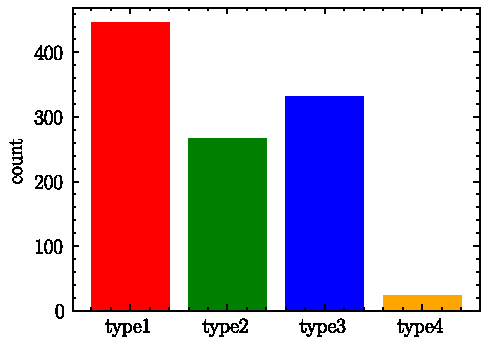
\includegraphics[width=.45\linewidth]{figure/RFM_count_bar.pdf}%
    \label{fig:wellclassbar}}
    \hfil
    \subfloat[RFM维度图]{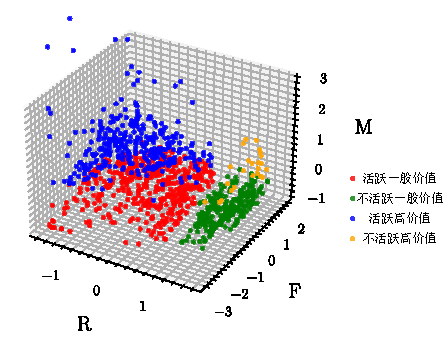
\includegraphics[width=.45\linewidth]{figure/RFM_scatter.pdf}%
    \label{fig:wellclasssca}}
    \caption{气井分类结果(type1:活跃高价值 type2:不活跃高价值 type3:活跃一般价值 type4:不活跃一般价值)}
    \label{fig:classResusca}
\end{figure}
\section{产气量预测实验结果}
\subsection{评估指标}
为了验证本章所提出的基于transformer的气井产量预测算法的有效性,使用两个指标用于评估。其中一个是平均绝对误差(Mean Absolute Error, MAE),其可以衡量
预测值与实际值之间的平均绝对偏差。公式如式\eqref{eq:MAE}所示。
\begin{equation}
    MAE(y, y') = \frac{1}{n} \sum_{i=1}^{n} |y_i - y'_i|
    \label{eq:MAE}
\end{equation}
另一个常用误差指标为累计产量的相对误差,公式如式\eqref{eq:RCPE}所示。
\begin{equation}
    RCPE = \frac{\sum_{i=1}^{n} |y_i| - \sum_{i=1}^{n} |y'_i|}{\sum_{i=1}^{n} |y_i|}
    \label{eq:RCPE}
\end{equation}
上面两式中,$i$表示索引,用于遍历数据集中的每一个数据点。例如,如果我们有一个包含多个观测值的数据集,$i$就用来表示这些观测值的序号,从第一个观测值
到第$n$个观测值。$y$表示真实值,也就是实际产量,$\hat{y}$表示预测值,也就是通过模型预测得到的产量。

\subsection{对比实验}
(1)分类预测与不分类预测对比

本次实验将气井分类之后再预测和不分类直接预测进行对比,其对比结果如表\ref{tab:classvalid}所示。为对比是否分类对预测结果的影响,使用本文模型针对未来7天的产气量构建预测模型,分别对每类型井的预测指标和不分类直接进行预测的结果进行统计,使用每类型气井预测结果的中位数作为对
该类预测效果的近似表示。
\begin{table}[H]
    \caption{分类预测与不分类预测结果对比}
    \label{tab:classvalid}
    \begin{tblr}{hlines,vlines,
        columns = {valign=m,co=-1},
        rows    = {halign=c},
        cell{1}{1} = {r=2}{c},
        cell{1}{2} = {c=2}{c},
        cell{1}{4} = {c=2}{c},
        cell{3}{2} = {r=4}{c},
        cell{3}{3} = {r=4}{c}
        }
        气井类别 & 不分类 & & 分类 & \\
          & MAE & RCPE & MAE & RCPE \\
        活跃高价值 & 0.477 & 0.058 & 0.225 & 0.030 \\
        不活跃高价值 & & & 0.367 & 0.051 \\
        活跃一般价值 & & & 0.103 & 0.042  \\
        不活跃一般价值 & & & 0.122 & 0.163  \\
    \end{tblr}
\end{table}
由表中可以看出,在不分类的情况下,预测结果的平均绝对误差(MAE)是0.477,相对百分比误差(RCPE)是0.058。除了不活跃一般价值的RCPE值高于不分类情况下的RCPE以外,这两个值在其他情况下均大于对每一类气井分别进行预测的结果。说明在进行气井产量预测时,先对气井进行分类再进行产气量预测在一定情况下时会达到比较好的效果的。

(2)消融实验
为了验证文中提出的基于Transformer模型中加入时间特征处理层和时域注意力层的有效性,本文对该算法设置消融实验来进行验证。将只加入时间特征处理层、只加入时域注意力层、两者都没有加的模型以及两者都加的模型(本文)在文中数据集上进行训练,
使用其针对未来七天的产气量进行预测,用结果指标的中位值来近视表示其预测结果。本文所得到的实验结果为对所有气井分类后,再按照气井的数量加权得到的。最终结果如表\ref{tab:ablation}所示。
\begin{table}[H]
    \caption{消融实验结果表}
    \label{tab:ablation}
    \begin{tblr}{hlines,vlines,
        columns = {valign=m,co=-1},
        rows    = {halign=c},}
        算法 & MAE & RCPE \\
        两者都无 & 0.736 & 0.377 \\
        仅无时域注意力层 & 0.436 & 0.113 \\
        仅无时间特征处理层 & 0.534 & 0.266 \\
        本文模型 & 0.220 & 0.042 \\
    \end{tblr}
\end{table}
由表中可知,将两个模块都去掉以后,模型的预测结果将显著下降,时间特征处理层对模型准确率的影响大于时域注意力层,这可能是由于气井产气量数据不具备明显的周期性,十分依赖过去的数据导致的。

(3) 对比模型选择

根据前文所述,本问题需要同时对1000余口气井构建时间序列预测模型,且问题包含多种类型的协变量,因此初步选取基于注意力机制的seq2seq模型,lightGBM模型、TFT模型以及本文的模型这四个可以解决这类问题的模型进行实验。

经过对手头的单井日报数据进行处理,累计10年,1000余口气井约有总共约有160多万条数据。为了展示各算法的预测性能,选取数量最多的一类井活跃高价值的产量数据作为测试集进行测试。如表\ref{fig:modelselection}所示,基于注意力机制的seq2seq模型,
由于模型结构限制,无法包含未来时刻的开关井信息,导致预测效果显著劣于其余三个模型。
lightGBM模型、TFT模型及本模型,预测准确率相近,本文算法略优于TFT和lightGBM模型,预测时间本文模型优于TFT和lightGBM模型。但是在模型训练阶段,lightGBM模型(10min)显著快于TFT模型(4h)及本文(2.5h)。故最终保留
本文中的模型和lightGBM模型。
\begin{table}[H]
    \caption{模型选择实验结果}
    \label{fig:modelselection}
    \begin{tblr}{hlines,vlines,
        columns = {valign=m,co=-1},
        rows    = {halign=c},
        cell{2}{1} = {r=4}{c}}
        测试对象 & 模型 & MAE($10^4 \ m^3$) & RCPE(\%)& 预测时间(s)\\ 
        活跃高价值气井& TFT          & 0.241                       & 3.14              & 8.369         \\       
                                    & LightGBM     & 0.262                       & 3.80              & 0.89     \\            
                                    & Seq2seq      & 0.512                       & 10.25             & 5.25   \\             
                                    & Ours         & 0.225                       & 3.02              & 7.29 \\               
    \end{tblr}
    % \centering
    % \begin{tabular}{|c|c|c|c|c|}
    %     \hline
    %     \textbf{测试对象} & \textbf{模型} & \textbf{MAE($10^4 \ m^3$)} & \textbf{RCPE(\%)} & \textbf{预测时间(s)} \\ \hline
    %     \multirow{4}{*}{活跃高价值气井}  & TFT          & 0.241                       & 3.14              & 8.369                \\ \cline{2-5}
    %                                 & LightGBM     & 0.262                       & 3.80              & 0.89                 \\ \cline{2-5}
    %                                 & Seq2seq      & 0.512                       & 10.25             & 5.25                 \\ \cline{2-5}
    %                                 & Ours         & 0.225                       & 3.02              & 7.29                 \\ \hline
    % \end{tabular}
\end{table}
结合图中可以看出,本文的模型在MAE和RCPE指标上的表现均优于其他三种模型,TFT由于参数量太复杂训练和预测时间都较久,效果也稍次于本模型。相对而言,LightGBM模型预测时间较短且也可以取得相对较好的预测结果。
这表明在实时性要求较高的场景中,LightGBM模型可能是一个较好的选择。Seq2seq模型在这三个测试对象上的表现相对较差,可能需要进一步优化模型结构或参数。根据实验结果,可以得出结论:在这三个测试对象上,本模型的预测性能最佳,
但预测时间较长。当实时性要求较高时,可以考虑使用LightGBM模型。

(4)使用部分数据进行预测

本次实验的动机为:由于早期数据缺乏套压记录,这可能会影响预测模型的准确性。近期数据包含了所有重要特征,包括套压数据,并且能够代表整个时间序列的主要趋势和模式,那么只使用近期数据进行预测可能是一个合理的选择。
\begin{table}[h]
    \renewcommand{\arraystretch}{1.5}
    \centering
    \caption{使用部分数据集训练和使用全数据集训练的对比}
    \label{tab:alldatacomparison}
    \begin{tabular}{|c|c|c|c|c|}
    \hline
    \textbf{气井类别} & \multicolumn{2}{c|}{{MAE}} & \multicolumn{2}{c|}{{RCPE}} \\ 
    \cline{2-5} 
    \textbf{(}$10^4 m^3$\textbf{)} & 使用部分数据 & 使用全部数据 & 使用部分数据 & 使用全部数据 \\ 
    \hline
    活跃高价值               & 0.193        & 0.225       & 0.023        & 0.030        \\ 
    \hline
    不活跃高价值               & 0.267        & 0.367        & 0.022        & 0.051        \\ 
    \hline
    活跃一般价值               & 0.101        & 0.103        & 0.047        & 0.042        \\ 
    \hline
    不活跃一般价值               & 0.120        & 0.122        & 0.165        & 0.163        \\ 
    \hline
    \end{tabular}
\end{table}
为对比预测效果,使用本文模型针对未来7天的产气量构建预测模型,分别使用所有数据和使用2017-01-01之后的数据构建两个不同的模型。根据分类结果将模型划分为四类,使用上文选定的两种模型对这5类型的气井分别进行预测。

    
通过对每类型气井的预测指标进行统计,可以得出以下结论:

对于活跃高价值的气井,使
用2017-01-01之后的数据预测的MAE为0.193,而使用所有数据的MAE为0.225。其RCPE分别为0.028和0.030。这说明基于2017-01-01之后的数据构建的模型预测效果较好。对于不活跃高价值的气井,使用2017-01-01之后的数据预测的MAE为0.267,使用所有数据的MAE为0.367。其RCPE分别为0.022和0.051。这说明对不活跃高价值气井而言,基于2017-01-01之后的数据构建的模型预测效果较好。
对于活跃一般价值的气井,使用2017-01-01之后的数据预测的MAE为0.101,而使用所有数据的MAE为0.103。其RCPE分别为0.047和0.042。对这类气井而言,基于2017-01-01之后的数据构建的模型在MAE上略好,总体来看,这两个模型的预测效果相当。
对于不活跃一般价值的气井,使用2017-01-01之后的数据预测的MAE为0.120,而使用所有数据的MAE为0.122。同时,RCPE分别为0.165和0.163。对于这类气井而言,基于所有数据构建的模型在RCPE上略好,但综合两个指标来看,两个模
型的预测效果相当。

综上所述,在大部分气井类别中,基于2017-01-01之后的数据构建的模型预测效果都较好。

(5)本模型和LightGBM模型对比

实验基本设置: 在这个实验中,我们选用本模型和LightGBM对未来7天的产气量进行预测。实验结果是对属于该日均产气量范围内的所有气井进行预测并计算其指标的中位数统计值得到的。
\begin{table}[H]
    \renewcommand{\arraystretch}{1.5}
    \centering
    \caption{本文模型和LightGBM模型预测结果对比}
    \label{tab:prediction_comparison}
    \begin{tabular}{|c|c|c|c|}
    \hline
    模型     & 气井种类 & MAE($10^4 m^3$) & RCPE(\%) \\ \hline
    LightGBM & 活跃高价值       &0.234            & 0.042 \\ \hline
    LightGBM & 不活跃高价值     & 0.341           & 0.066    \\ \hline
    LightGBM & 活跃一般价值      & 0.136           & 0.093    \\ \hline
    LightGBM & 不活跃一般价值      & 0.128           & 0.228    \\ \hline
    Ours      & 活跃高价值        &0.225            &0.030      \\ \hline
    Ours      & 不活跃高价值      & 0.367           & 0.051   \\ \hline
    Ours      & 活跃一般价值      & 0.103           & 0.042    \\ \hline
    Ours      &不活跃一般价值      & 0.122           & 0.163    \\ \hline
    \end{tabular}
\end{table}

实验结果对比与分析: 根据上述统计结果表格,可以看出:

对于不活跃一般价值的气井,本文模型的MAE和RCPE分别为0.122和0.163,而LightGBM模型分别为0.128和0.228。对于这类气井而言,本文模型的预测性能更好。
对于活跃一般价值的气井,本文模型的MAE和RCPE分别为0.103和0.042,而LightGBM模型分别为0.136和0.093。在这种情况下,本文模型的预测性能也更好。
对于不活跃高价值的气井,本文模型的MAE和RCPE分别为0.367和0.051,而LightGBM模型分别为0.341和0.066。在这种情况下,尽管本文模型在RCPE上的表现更好,但在MAE上,LightGBM模型的表现更优。
对于活跃高价值的气井, 本文模型的MAE和RCPE分别为 0.225和0.030,而LiGBM模型分别为0.234和0.042。对于这类井而言,依然是本文模型的预测性能更好。

从预测性能上看,本文模型在各种情况下都表现出较好的预测性能。然而,从时间角度来看,LightGBM模型的训练和预测时间要远远低于本文模型。具体来说,LightGBM模型的重训练时间为5分钟,而本文模型为1小时;LightGBM模型
的预测时间平均约为1.2秒,而本文模型平均约为7.5秒。这意味着,在实际应用中,使用LightGBM模型会更加节省时间和计算资源。

总结:从实验结果来看,本文模型在预测性能上具有优势,但在时间方面,LightGBM模型具有更好的表现。因此,在实际应用中,需要根据实际需求的精度和计算资源进行权衡,选择合适的模型。
\subsection{实验结果统计值展示}
为完整展示实验结果,分别列出两种预测模型分别在预测步长为7天和45天时的预测结果统计指标,统计指标不仅包括中位数,还包括平均数,\%25分位数,75\%分位数,标准差。此处取所有分类结果的均值。预测步长7天的MAE结果如表\ref{tab:MAE7}所示。
\begin{table}[H]
    \renewcommand{\arraystretch}{1.5}
    \centering
    \caption{本文模型和LightGBM模型预测未来7天内产气量预测结果的MAE指标对比}
    \label{tab:MAE7}
    \begin{tabular}{|c|c|c|c|c|c|c|}
    \hline
    模型     & 气井类别 & MAE mean & MAE std & MAE 25\% & MAE 50\% & MAE 75\% \\ \hline
    LightGBM  &活跃高价值       &0.203     & 0.248   & 0.063    & 0.131     &0.244 \\ \hline 
    LightGBM & 不活跃高价值      & 0.279    & 0.366   & 0.087    & 0.163    & 0.297    \\ \hline
    LightGBM & 活跃一般价值     & 0.180    & 0.179   & 0.069    & 0.136    & 0.211    \\ \hline
    LightGBM & 不活跃一般价值      & 0.199    & 0.269   & 0.055    & 0.128    & 0.277    \\ \hline
    Ours      & 活跃高价值         & 0.189    &0.227    &0.059     & 0.134     &1.239  \\ \hline
    Ours       & 不活跃高价值      & 0.287    & 0.309   & 0.089    & 0.149    & 0.298    \\ \hline
    Ours      & 活跃一般价值     & 0.170    & 0.220   & 0.061    & 0.102    & 0.186    \\ \hline
    Ours     & 不活跃一般价值     & 0.174    & 0.236   & 0.053    & 0.122    & 0.205    \\ \hline
    \end{tabular}
\end{table}
预测步长7天的RCPE结果如表\ref{tab:RCPE7}所示。
\begin{table}[H]
    \renewcommand{\arraystretch}{1.5}
    \centering
    \caption{本文模型和LightGBM模型预测未来7天内产气量预测结果的RCPE指标对比}
    \label{tab:RCPE7}
    \begin{tabular}{|c|c|c|c|c|c|c|} % Change 'l' to 'c' for center alignment
    \hline
    模型     & 气井类别 & RCPE mean & RCPE std & RCPE 25\% & RCPE 50\% & RCPE 75\% \\ \hline
    LightGBM & 活跃高价值        &0.105     & 0.139     &0.029      0.053       &0.113 \\ \hline
    LightGBM & 不活跃高价值      & 0.085     & 0.125    & 0.020     & 0.043     & 0.094     \\ \hline
    LightGBM & 活跃一般价值     & 0.131     & 0.147    & 0.038     & 0.093     & 0.167     \\ \hline
    LightGBM & 不活跃一般价值      & 0.433     & 0.845    & 0.097     & 0.228     & 0.477     \\ \hline
    Ours      &活跃高价值         &0.093     & 0.128     &0.022      & 0.031      &0.103 \\ \hline
    Ours      & 不活跃高价值      & 0.086     & 0.119    & 0.015     & 0.035     & 0.080     \\ \hline
    Ours      & 活跃一般价值     & 0.112     & 0.187    & 0.016     & 0.047     & 0.098     \\ \hline
    Ours      & 不活跃一般价值      & 0.363     & 0.757    & 0.066     & 0.163     & 0.358     \\ \hline
    \end{tabular}
\end{table}
预测步长45天的MAE结果如表\ref{tab:MAE45}所示。
\begin{table}[H]
    \renewcommand{\arraystretch}{1.5}
    \centering
    \caption{本文模型和LightGBM模型预测未来45天内产气量预测结果的MAE指标对比}
    \label{tab:MAE45}
    \begin{tabular}{|c|c|c|c|c|c|c|}
    \hline
    模型       & 气井类别 & MAE mean & MAE std & MAE 25\% & MAE 50\% & MAE 75\% \\ \hline
    LightGBM  & 活跃高价值        & 0.203   & 0.174    &0.098    & 0.178     & 0.298 \\ \hline
    LightGBM  & 不活跃高价值      & 0.360    & 0.329   & 0.151    & 0.253    & 0.418    \\ \hline
    LightGBM  & 活跃一般价值     & 0.245    & 0.191   & 0.106    & 0.186    & 0.306    \\ \hline
    LightGBM  & 不活跃一般价值      & 0.198    & 0.151   & 0.091    & 0.159    & 0.273    \\ \hline
    Ours       & 活跃高价值        &0.153     & 0.188   & 0.069     & 0.128   & 0.233   \\ \hline
    Ours       & 不活跃高价值      & 0.346    & 0.319   & 0.111    & 0.245    & 0.459    \\ \hline
    Ours       & 活跃一般价值     & 0.217    & 0.207   & 0.077    & 0.130    & 0.272    \\ \hline
    Ours       & 不活跃一般价值      & 0.132    & 0.113   & 0.058    & 0.110    & 0.181    \\ \hline
    \end{tabular}
\end{table}
预测步长45天的RCPE结果如表\ref{tab:RCPE45}所示。 
\begin{table}[H]
    \renewcommand{\arraystretch}{1.5}
    \centering
    \caption{本文模型和LightGBM模型预测未来45天内产气量预测结果的RCPE指标对比}
    \label{tab:RCPE45}
    \begin{tabular}{|c|c|c|c|c|c|c|}
    \hline
    模型       & 气井类别 & RCPE mean & RCPE std & RCPE 25\% & RCPE 50\% & RCPE 75\% \\ \hline
    LightGBM  & 活跃高价值       & 0.085      &0.097    &0.023      &0.051      & 0.104 \\ \hline
    LightGBM  & 不活跃高价值      & 0.091     & 0.107    & 0.028     & 0.056     & 0.114     \\ \hline
    LightGBM  & 活跃一般价值     & 0.117     & 0.121    & 0.029     & 0.074     & 0.160     \\ \hline
    LightGBM  & 不活跃一般价值      & 0.384     & 0.750    & 0.089     & 0.201     & 0.396     \\ \hline
    Ours       &活跃高价值          & 0.073    0.089      & 0.017     & 0.042     & 0.109 \\ \hline
    Ours       & 不活跃高价值      & 0.087     & 0.094    & 0.019     & 0.047     & 0.120     \\ \hline
    Ours       & 活跃一般价值     & 0.112     & 0.128    & 0.026     & 0.072     & 0.146     \\ \hline
    Ours       & 不活跃一般价值      & 0.361     & 0.731    & 0.071     & 0.146     & 0.319     \\ \hline
    \end{tabular}
\end{table}
为直观展示预测结果,选择6口气井的预测结果如下文所示。
\begin{figure}[H]
    \centering
    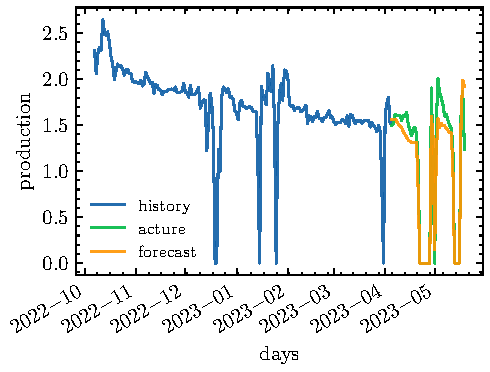
\includegraphics[width=.9\linewidth]{figure/forecast_SN0018-03.pdf}
    \caption{井XE8867-HU预测结果}
\end{figure}
\begin{figure}[H]
    \centering
    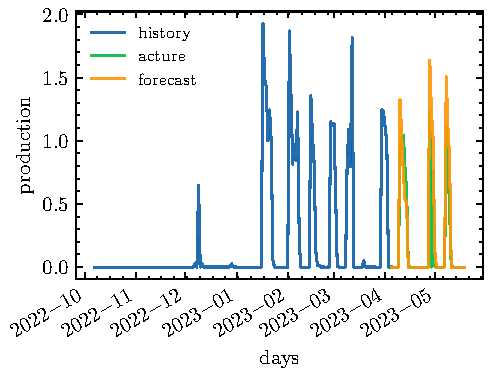
\includegraphics[width=.9\linewidth]{figure/forecast_SN0037-01.pdf}
    \caption{井XE3878-RE预测结果}
\end{figure}
\begin{figure}[H]
    \centering
    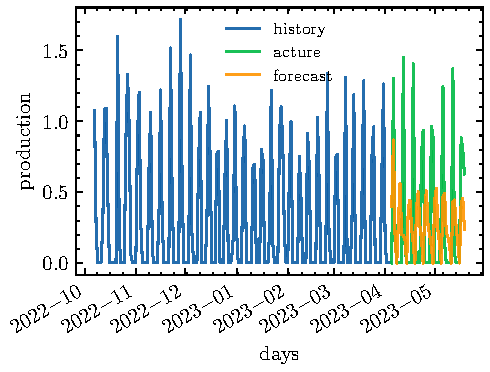
\includegraphics[width=.9\linewidth]{figure/forecast_SN0049-08.pdf}
    \caption{井SI2938-KI预测结果}
\end{figure}
\begin{figure}[H]
    \centering
    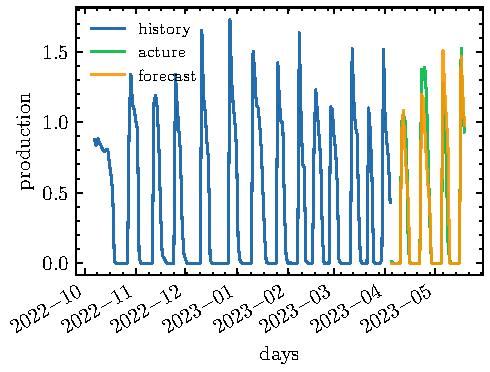
\includegraphics[width=.9\linewidth]{figure/forecast_SN0075-04ST.pdf}
    \caption{井HC8772-MA预测结果}
\end{figure}
\begin{figure}[H]
    \centering
    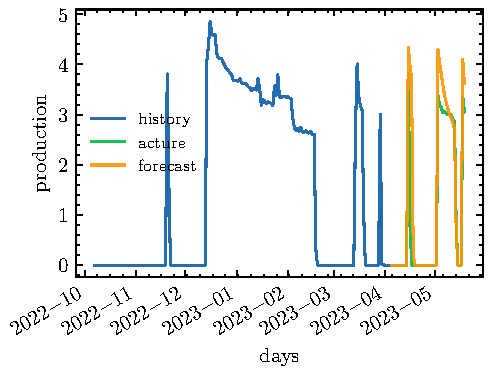
\includegraphics[width=.9\linewidth]{figure/forecast_SN0087-03i.pdf}
    \caption{井LR7359-BR预测结果}
\end{figure}
\begin{figure}[H]
    \centering
    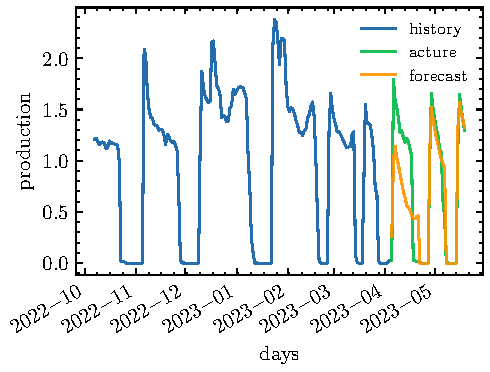
\includegraphics[width=.9\linewidth]{figure/forecast_SN0095-06.pdf}
    \caption{井RC8375-BN预测结果}
\end{figure}
\section{开关井推荐}
本小节将介绍开关井策略推荐实际问题的解决办法。首先收集数据,包括井口产气量、井底压力、温度、环境温度、气价、能源成本等相关参数。同时也需
要采集各个气井的位置和特征等信息,以便进行搜索和选择。其次,根据实际情况和目标函数,选择合适的搜索算法。常见的搜索算法包括深度优先搜索、蚁群算法等。
不同算法有不同的优缺点,需要根据实际情况进行评估和选择。然后确定搜索空间,搜索空间即可选取的所有井的集合,需要考虑到可行性和搜索效率的平衡。通常可
以根据实际条件和目标函数,设置一些限制条件来缩小搜索空间,以提高搜索效率。接下来要执行搜索算法,根据设定的搜索算法,对搜索空间进行搜索。在搜索过程
中,需要按照目标函数的要求,评估不同井进行开关的效果,并记录每次开关井的结果和成本。在搜索完成后,需要对所有开关井的结果进行评估,选取最优的开关井方案。
评估时需要考虑到产量、成本、环境、管网模型等多方面因素,并综合权衡不同因素的影响,以选取最优的开关井方案。最后根据最优的开关井方案,实施相应的开关井策略。

气井开采过程中,通常会产生一定量的液体,包括水和油。产液量的增加会影响气井的产气量,因为液体在井筒中的积累会增加井筒的阻力,使气流的速度降低,
从而影响气井的产气量。当气井处于低压低产阶段时,气相不能有效地携带液体,会导致积液现象。此时,如采用间歇生产方式(即周期性地开关井),可以利用
关闭期间积累的压力差,在开启时将积聚在底部或中部的液体迅速排出。
但如果开关频率过高或关闭时间过短,则可能造成反复积排液、增加摩阻损失、降低生产效率。可若是开关频率过低或关闭时间过长,则可能导致底部水锥突
破、增加水含率、降低天然气质量。
\subsection{数据}
本小节使用过去三十天的井口温度、压力、开关井时间、产气量值并借助前文训练的产气量模型来预测未来七天内每口井的预计产气量;本文使用前一天的井口温度、压力以
及井丛的拓扑关系图等数据构建管网模型,计算压力差;通过对过去一段时间历史数据的总结得到每口井的开关井周期。
\subsection{算法设计}

(1)管网模型

在处理复杂的地下流体动力学问题时,精确的解析解往往难以获得。在某些情况下,特别是考虑到地层的渗透性、流体的粘度以及井筒和储层之间的压力交互作用时,压力沿
井深的变化近似于二次曲线。此处在计算平均压力时根据此理论采用了一个简化的假设,即压力分布沿井深呈二次曲线分布。在这个假设下,可以通过连接干管井丛的井口压
力平均值(P1)和管道出口压力,即集气站进站压力(P2)计算出平均压力(avgPressure)。具体公式如式\eqref{eq:avgPressure}所示。
\begin{equation}
    \text{avgPressure} = \frac{2.0 \times (P1^3 - P2^3)}{3.0 \times (P1^2 - P2^2)}
    \label{eq:avgPressure}
\end{equation}
式中,P1 和 P2 分别代表两个不同深度的压力值。

本文使用了一种经验模型来计算临界温度(Tpc)和临界压力(Ppc)。这个模型是基于大量实验数据得出的,它将气体相对密度($\delta$ )作为输入参数。
\begin{equation}
    T_{pc} = 93.3 + 181 \times \delta - 7 \times \delta^2
\end{equation}
\begin{equation}
    P_{pc} = 4.668 + 0.103 \times \delta - 0.259 \times \delta^2
\end{equation}
式中的气体相对密度$\delta$的默认取值为0.5962(无量纲)。

将实际温度(K)和平均压力(avgPressure)分别除以临界温度(Tpc)和临界压力(Ppc),得到温度和压力的缩减值(即相对于临界温度和临界压力的温度和压力)Tr和Pr。
\begin{equation}
    T_r = \frac{K}{T_{pc}}
\end{equation}
\begin{equation}
    P_r = \frac{\text{avgPressure}}{P_{pc}}
\end{equation}
式中K为开尔文温度$K = C + 273.15$。

压缩因子(Z-factor)是一个描述气体实际体积与理论(理想气体状态下的)体积之比的参数,是用于石油和天然气工程中评估气体的压缩性质的重要工具。压缩因子的值表明了实际气体与理想气体状态方程之间的偏离程度。

赞达尔方程\cite{Dranchuk1975CalculationOZ}(也称为Dranchuk-Aboukassem方程),是一种基于实验数据得出的经验公式,用于计算特定条件下的气体压缩因子。这个方程考虑了温度和压力的缩减值。具体公式如式\eqref{eq:Z-factor}所示。
\begin{equation}
    Z = 1 - \frac{3.52 \times P_r}{10^{0.9813T_r}} + \frac{0.274 \times P_r \times P_r}{10^{0.8157T_r}}
    \label{eq:Z-factor}
\end{equation}
通过使用该方程,可以在已知缩减温度和缩减压力的情况下,估计出天然气在特定温度和压力条件下的压缩因子,进而帮助工程师们更准确地预测和计算气体的行为和性能。
本式对于理解和计算实际天然气在地下储藏和输送过程中的物理行为至关重要。它使工程师能够更好地设计和优化天然气的提取、处理和运输系统。

最后,可以使用Darcy-Weisbach方程\cite{brown2002history}来计算压力。这个方程描述了气体在管道中流动时,由于摩擦损失而引起的压力降。在这里,需要考虑到气体的压缩性,因此使用压缩因子(Z)来修正方程。
\begin{equation}
    \text{calP1} = \left(P2^2 + 3.948 \times 10^{-8} \times Q \times Q \times \delta \times K \times \frac{L}{d^{1.6}}\right)^{0.5}
\end{equation}
此处Q代表产气量,单位为万方/日,在计算中需要进行单位换算。d是气井的管径,单位为毫米,默认取值为20。
当应用场景为气井传输管道(从井丛传输至集气站)时,$calP1$和$P1 - calP1$具有以下实际意义。

$calP1$:这个值表示计算得到的管道起点(如单口气井)的压力。它反映了在给定的生产条件(温度、产气量等)以及管道参数(长度、直径等)下,为了克服管道摩擦损失所需要的起始压力。 

$P1 - calP1$:这个值表示实际管道起点压力(P1)与计算得到的起点压力($calP1$)之间的差值。这个差值可以用来评估管道的性能和系统效率。以下是几种可能的情况:

当$P1 - calP1$接近于零时,表示实际压力和计算压力非常接近,说明管道系统运行良好,摩擦损失在可接受范围内。 

当$P1 - calP1$为正值时,表示实际起点压力高于计算压力。这可能意味着管道系统存在过高的摩擦损失或是管道中存在堵塞等异常现象。 

当$P1 - calP1$为负值时,表示实际起点压力低于计算压力。这可能意味着管道系统效率较高,但也可能导致管道中的气体流量不足,从而影响到集气站的运行。 

通过分析$calP1$和$P1 - calP1$这两个值,可以为气井生产提供有用信息,有助于对生产参数进行调整和优化,提高气井生产效率和安全性。同时,这些信息也可以用于诊断管道系统是否存在异常,以便及时采取纠正措施。

(2)搜索算法

基于对实际问题的分析,借助FOA算法来完成搜索。
主要对FOA算法中的距离进行了自定义:

当目前产量$current\_amount>target$(预计想要达到的总产量),系统需要从开着的井中选择一口井关闭,这时认为距离函数与压力差$delta\_pressure$和已经开井时间$open\_time$高度相关,因此距离函数定义如\eqref{eq:closewell}所示。
\begin{equation}
    \text{Dist}_i = \frac{1}{\sqrt{{\text{delta\_pressure}_i}^2 + {\text{open\_time}_i}^2}}
    \label{eq:closewell}
\end{equation}
当目前产量$current\_amount<target$时,系统需要从可以开的井中选择一口井打开,本文认为压力差越小越好,产气量越大越好,因此距离函数与产气量、压力差有关,距离函数的定义如如\eqref{eq:openwell}
\begin{equation}
    \text{Dist}_i = \frac{\sqrt{{\text{delta\_pressure}_i}^2}}{\sqrt{{\text{pre\_production}_i}^2}}
    \label{eq:openwell}
\end{equation}
将当前问题代入到果蝇优化算法具体的步骤如\ref{al:openwell}所示。
\begin{algorithm}[H]
    \caption{基于果蝇优化的开关井推荐算法}
    \begin{algorithmic}[1]
       \Require 目标产气量target区间,前一天的开关井情况
       \Ensure  新的开关井策略
       \State 初始化,以第一天的开关井情况作为初始值 init()
       \While{true}
            \If{current\_amount $>$ target}
                \State 随机分配方向、距离,搜索出一定数量可以关的井 update()
            \ElsIf{current\_amount $<$ target}
                \State 随机分配方向、距离,搜索出一定数量可以开的井 update()
            \Else
                \State \Return 最终开关井策略
            \EndIf
            \State 计算自定义的种群适应度
            \State 果蝇位置更新
        \EndWhile
    \end{algorithmic}
    \label{al:openwell}
\end{algorithm}

(3)搜索空间

在实际生产过程中,不是所有的关着井都可以开,需要动态的挑出这些可以开的井。根据分析,本文排除下面这些井,在这个周期不投入生产。

1.去除用户前端自定义输入的尚不参与生产的井;

2.根据历史数据计算开关井周期,如果某口井当前已经开井时间大于最大开井时间,则排除这口井;

3.基于管网模型计算压力差,并根据用户输入阈值去除压力差过大的井;

4.单口井的生产能力太低的井。
(4)
